\documentclass[xcolor={dvipsnames,table},aspectratio=169]{beamer}
\usepackage[utf8]{inputenc}
\usepackage[T1]{fontenc}
\usepackage[brazil]{babel}
\usepackage{graphics,amssymb,amsfonts,amsmath}
\usepackage{tikz}
\usepackage{enumerate,hyperref}
\usepackage{palatino}
\usepackage{ragged2e}
\usepackage{minted}
\usepackage{booktabs}
\usepackage{verbatim}
\usepackage[export]{adjustbox}
\usepackage{tikz}                   
\usepackage{xcolor}
\usepackage{textcomp} % para usar \textdegree
\usetikzlibrary{shadows}
\usetheme{AnnArbor}
\usecolortheme{orchid}
\usefonttheme[onlymath]{serif}

\AtBeginSection[]{
  \begin{frame}
  \vfill
  \centering
  \begin{beamercolorbox}[sep=8pt,center,shadow=true,rounded=true]{title}
    \usebeamerfont{title}\insertsectionhead\par%
  \end{beamercolorbox}
  \vfill
  \end{frame}
}

\newminted{java}{bgcolor=cyan!10}

\newcolumntype{C}[1]{>{\centering\let\newline\\\arraybackslash\hspace{0pt}}m{#1}}

\title[\sc{Métodos}]{Métodos}
\author[Roland Teodorowitsch]{Roland Teodorowitsch}
\institute[FPROG - EP - PUCRS]{Fundamentos de Programação - Escola Politécnica - PUCRS}
\date{26 de outubro de 2022}

\begin{document}
\justifying

%-------------------------------------------------------
\begin{frame}
	\titlepage
\end{frame}

%=======================================================
\section{Introdução}

%-------------------------------------------------------
\begin{frame}\frametitle{Objetivos}
\begin{itemize}
	\item Ser capaz de implementar métodos
	\item Tornar-se familiar com o conceito de passagem de parâmetros
	\item Desenvolver estratégias para decomposição de tarefas complexas em tarefas mais simples
	\item Ser capaz de determinar o escopo de variáveis
	\item Aprender como pensar recursivamente
\end{itemize}
\end{frame}

%-------------------------------------------------------
\begin{frame}\frametitle{Conteúdos}
\begin{itemize}
	\item Métodos como Caixas Pretas
	\item Implementando Métodos
	\item Passagem de Parâmetros
	\item Retorno de Valores
	\item Métodos sem Retorno de Valores
	\item Solução de Problemas
	\begin{itemize}
		\item Reutilização de Métodos
		\item Refinamento Passo-a-passo
	\end{itemize}
	\item Escopo de Variáveis
	\item Métodos Recursivos
\end{itemize}
\end{frame}

%=======================================================
\section{Métodos como Caixas Pretas}

%-------------------------------------------------------
\begin{frame}[fragile]\frametitle{Métodos como Caixas Pretas}
\begin{itemize}
	\item Um método é uma sequência de instruções com um nome
	\begin{itemize}
		\item Você declara um método definindo um bloco de código com nome
\begin{javacode}
public static void main(String[] args) {
  double result = Math.pow(2, 3);
  . . .
}
\end{javacode}
		\item Você chama o método de forma a executar as suas instruções
	\end{itemize}
	\item Um método empacota uma computação formada por múltiplos passos em uma forma que pode ser facilmente entendida e reutilizada.
\end{itemize}
\end{frame}

%-------------------------------------------------------
\begin{frame}\frametitle{O que é um Método?}
\begin{itemize}
	\item Você já utilizou alguns métodos:
	\begin{itemize}
		\item \texttt{Math.pow()}
		\item \texttt{String.length()}
		\item \texttt{Character.isDigit()}
		\item \texttt{Scanner.nextInt()}
		\item \texttt{main()}
	\end{itemize}
	\item Eles têm:
	\begin{itemize}
		\item Um nome de método: seguindo as mesmas regras de nomes de variáveis (estilo camelHump)
		\item Um par de parênteses ao seu final, para fornecer informação (argumentos) para a sua execução
	\end{itemize}
\end{itemize}
\end{frame}

%-------------------------------------------------------
\begin{frame}[fragile]\frametitle{Fluxograma da Chamada de um Método}
\begin{columns}[T]
	\begin{column}{0.5\linewidth}
\begin{figure}[h]
	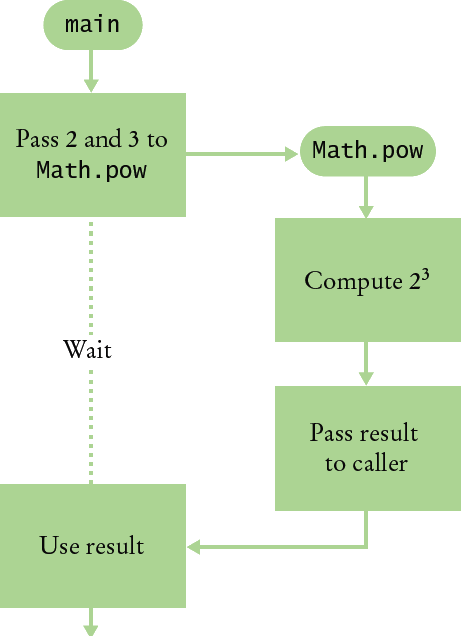
\includegraphics[height=0.65\paperheight,center]{pucrs-ep-fprog-unidade_05-metodos-laminas-fluxograma_metodo.png}
\end{figure}
	\end{column}
	\begin{column}{0.5\linewidth}
{\scriptsize
\begin{javacode}
public static void main(String[] args) {
  double result = Math.pow(2, 3);
  ...
}
\end{javacode}
}
		\begin{itemize}
			\item Um método ``chama'' outro
			\begin{itemize}
				\item \texttt{main} chama \texttt{Math.pow()}
				\item Dois argumentos são passados: 2 e 3
				\item \texttt{Math.pow} inicia
				\begin{itemize}
					\item Usa os argumentos (2, 3)
					\item Faz o seu trabalho
					\item Retorna a resposta
				\end{itemize}
				\item \texttt{main} usa o resultado
			\end{itemize}
		\end{itemize}
	\end{column}
\end{columns}
\end{frame}

%-------------------------------------------------------
\begin{frame}[fragile]\frametitle{Valores de Argumentos e Retorno}
\begin{columns}[T]
	\begin{column}{0.5\linewidth}
{\scriptsize
\begin{javacode}
public static void main(String[] args) {
  double result = Math.pow(2,3);
  . . .
}
\end{javacode}
}
		\begin{itemize}
			\item \texttt{main} ``passa'' dois argumentos (2 e 3) para \texttt{Math.pow}
			\item \texttt{Math.pow} calcula e retorna o valor 8 para \texttt{main}
			\item \texttt{main} armazena o valor de retorno na variável \texttt{result}
		\end{itemize}
	\end{column}
	\begin{column}{0.5\linewidth}
\begin{figure}[h]
	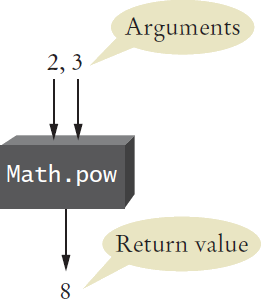
\includegraphics[height=0.5\paperheight,center]{pucrs-ep-fprog-unidade_05-metodos-laminas-argumentos_e_retorno.png}
\end{figure}
	\end{column}
\end{columns}
\end{frame}

%-------------------------------------------------------
\begin{frame}\frametitle{Analogia com uma Caixa Preta}
\begin{itemize}
	\item Um termostato é uma ``caixa preta''
	\begin{itemize}
		\item Defina a termperatura desejada
		\item O termostato liga o aquecimento conforme necessário
		\item Não é preciso saber como ele realmente funciona!
		\begin{itemize}
			\item Como ele sabe a temperatura corrente?
			\item Quais sinais/comandos ele deve enviar ao aquecedor para ligá-lo?
		\end{itemize}
	\end{itemize}
	\item Use métodos como ``caixas pretas''
	\begin{itemize}
		\item Passe para o método o que ele precisa para fazer o seu trabalho
		\item Receba a resposta
	\end{itemize}
\end{itemize}
\end{frame}

%=======================================================
\section{Implementando Métodos}

%-------------------------------------------------------
\begin{frame}[fragile]\frametitle{Implementando Métodos}
\begin{itemize}
	\item Um método para calcular o volume de um cubo
	\begin{itemize}
		\item O que ele precisa para fazer os seu processamento?
		\item Qual resposta ele retorna?
	\end{itemize}
	\item Quando se escreve um método:
	\begin{itemize}
		\item Escolha um nome para o método (\texttt{cubeVolume})
		\item Declare uma variável para cada argumento de entrada \texttt{(double sideLength)}
		\item Determine o tipo do valor retornado (\texttt{double})
		\item Adicione modificadores tais como \texttt{public static}
	\end{itemize}
\begin{javacode}
public static double cubeVolume(double sideLength)
\end{javacode}
\end{itemize}
\end{frame}

%-------------------------------------------------------
\begin{frame}[fragile]\frametitle{Dentro do Método}
\begin{itemize}
	\item Escreva o corpo do método
	\begin{itemize}
		\item O corpo do método é colocado entre chaves
		\item O corpo contém declarações de variáveis e comandos que são executados quando o método é chamado
		\item O método também deve retornar o valor calculado
	\end{itemize}
\begin{javacode}
public static double cubeVolume(double sideLength) {
  double volume = sideLength * sideLength * sideLength;
  return volume;
}
\end{javacode}
\end{itemize}
\end{frame}

%-------------------------------------------------------
\begin{frame}[fragile]\frametitle{Fora do Método}
\begin{itemize}
	\item Os valores retornados por \texttt{cubeVolume} são armazenados em variáveis locais dentro de \texttt{main}
	\item Os resultados são mostrados
{\scriptsize
\begin{javacode}
public static void main(String[] args) {
   double result1 = cubeVolume(2);
   double result2 = cubeVolume(10);
   System.out.println("A cube of side length 2 has volume "  + result1);
   System.out.println("A cube of side length 10 has volume " + result2);
}
\end{javacode}
}
\end{itemize}
\end{frame}

%-------------------------------------------------------
\begin{frame}\frametitle{Sintaxe da Declaração de Métodos}
\begin{figure}[h]
	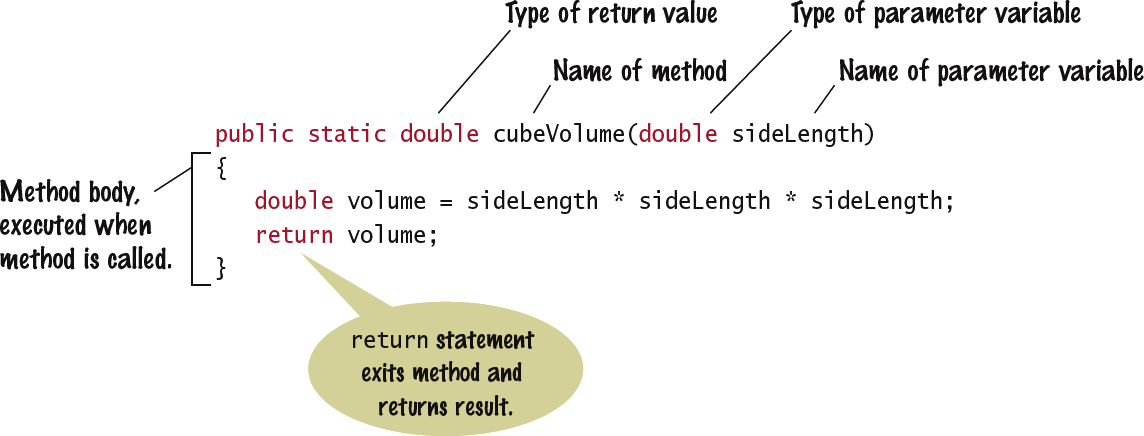
\includegraphics[height=0.65\paperheight,center]{pucrs-ep-fprog-unidade_05-metodos-laminas-sintaxe_metodos.png}
\end{figure}
\end{frame}

%-------------------------------------------------------
\begin{frame}[fragile]\frametitle{\texttt{Cubes.java} {\tiny (HORSTMANN, 2013, p. 206)}}
{\tiny
\begin{javacode}
/**
   This program computes the volumes of two cubes.
*/
public class Cubes {
   public static void main(String[] args) {
      double result1 = cubeVolume(2);
      double result2 = cubeVolume(10);
      System.out.println("A cube with side length 2 has volume " + result1);
      System.out.println("A cube with side length 10 has volume " + result2);
   }

   /**
      Computes the volume of a cube.
      @param sideLength the side length of the cube
      @return the volume
   */
   public static double cubeVolume(double sideLength) {
      double volume = sideLength * sideLength * sideLength;
      return volume;
   }
}
\end{javacode}
~\\
~\\
\textbf{Resultado da execução:}\\
\texttt{A cube with side length 2 has volume 8\\
A cube with side length 10 has volume 1000\\}
}
\end{frame}

%-------------------------------------------------------
\begin{frame}[fragile]\frametitle{Comentários de Métodos}
\begin{itemize}
	\item Escreva um comentário Javadoc acima de cada método
	\item Inicie com \texttt{/**}
	\begin{itemize}
		\item Indique o propósito do método
		\item Descreva cada argumento de entrada com \texttt{@param}
		\item Descreva o valor de retorno com \texttt{@return}
	\end{itemize}
	\item Termine com \texttt{*/}
\begin{javacode}
/**
  Computes the volume of a cube.
  @param sideLength the side length of the cube
  @return the volume
*/
public static double cubeVolume(double sideLength)
\end{javacode}
\end{itemize}
\end{frame}

%=======================================================
\section{Passagem de Parâmetros}

%-------------------------------------------------------
\begin{frame}\frametitle{Passagem de Parâmetros}
\begin{columns}[T]
	\begin{column}{0.7\linewidth}
\begin{itemize}
	\item Variáveis de parâmetros recebem os valores dos argumentos fornecidos na chamada do método
	\begin{itemize}
		\item Ambos devem ser do mesmo tipo
	\end{itemize}
	\item O valor do \textbf{argumento} (parâmetro real) pode ser:
	\begin{itemize}
		\item O conteúdo de uma variável
		\item Um valor constante
		\item Uma expressão
	\end{itemize}
	\item \textbf{Variáveis de parâmetros} (parâmetros formais) são
	\begin{itemize}
		\item Declaradas no método chamado
		\item Inicializadas com o valor do argumento
		\item Usadas como variáveis dentro do método chamado
	\end{itemize}
\end{itemize}
	\end{column}
	\begin{column}{0.3\linewidth}
\begin{figure}[h]
	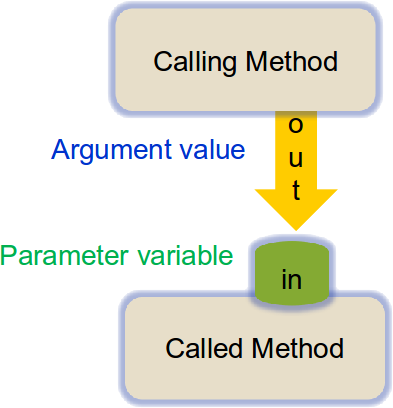
\includegraphics[height=0.5\paperheight,center]{pucrs-ep-fprog-unidade_05-metodos-laminas-passagem_de_parametros.png}
\end{figure}
	\end{column}
\end{columns}
\end{frame}

%-------------------------------------------------------
\begin{frame}[fragile]\frametitle{Passos da Passagem de Parâmetros}
{\tiny
\begin{javacode}
public static void main(String[] args) {
  double result1 = cubeVolume(2);
  . . . 
}
\end{javacode}
\begin{figure}[h]
	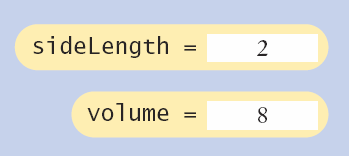
\includegraphics[height=0.12\paperheight,center]{pucrs-ep-fprog-unidade_05-metodos-laminas-passo_passagem_de_parametros_1.png}
\end{figure}
\begin{javacode}
public static double cubeVolume(double sideLength) {
  double volume = sideLength * sideLength * sideLength;
  return volume;
}
\end{javacode}
\begin{figure}[h]
	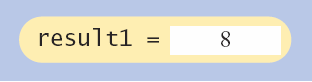
\includegraphics[height=0.08\paperheight,center]{pucrs-ep-fprog-unidade_05-metodos-laminas-passo_passagem_de_parametros_2.png}
\end{figure}
\begin{javacode}
public static void main(String[] args) {
  double result1 = cubeVolume(2);
  . . . 
}
\end{javacode}
}
\end{frame}

%-------------------------------------------------------
\begin{frame}[fragile]\frametitle{Erro Comum}
Erro comum = tentar modificar argumentos
\begin{itemize}
	\item Uma cópia do argumento é passada para o método
	\item O método chamado pode modificar cópias locais dos parâmetros, mas não pode modificar o valor original
{\small
\begin{javacode}
public static void main(String[] args) {
  double total = 10;
  addTax(total, 7.5); 
}

public static int addTax(double price, double rate) {
  double tax = price * rate / 100;
  price = price + tax; // NAO tem efeito fora do metodo
  return tax;
}
\end{javacode}
}
\end{itemize}
\end{frame}

%=======================================================
\section{Retorno de Valores}

%-------------------------------------------------------
\begin{frame}[fragile]\frametitle{Retorno de Valores}
\begin{itemize}
	\item Métodos podem (opcionalmente) retornar um valor
	\begin{itemize}
		\item Declare um tipo de retorno na declaração do método
		\item Adicione um comando \texttt{return} que retorna um valor
		\item O comando \texttt{return} faz duas coisas
		\begin{itemize}
			\item Termina imediatamente o método
			\item Passa o valor de retorno de volta para a chamada do método
		\end{itemize}
		\item O valor de retorno pode ser uma constante, uma variável ou o cálculo de uma expressão, mas precisa corresponder ao tipo de retorno declarado
	\end{itemize}
\begin{javacode}
public static double cubeVolume (double sideLength) {
  double volume = sideLength * sideLength * sideLength;
  return volume;
}
\end{javacode}
\end{itemize}
\end{frame}

%-------------------------------------------------------
\begin{frame}[fragile]\frametitle{Múltiplos Comandos \texttt{return}}
\begin{columns}[T]
	\begin{column}{0.7\linewidth}
\begin{itemize}
	\item Um método pode usar múltiplos comandos \texttt{return}
	\item Cada ramo de execução deve possuir um comando \texttt{return}
{\scriptsize
\begin{javacode}
public static double cubeVolume(double sideLength) {
  if (sideLength < 0) { 
    return 0; 
  }
  return sideLength * sideLength * sideLength;
}
\end{javacode}
}
\end{itemize}
	\end{column}
	\begin{column}{0.3\linewidth}
\begin{figure}[h]
	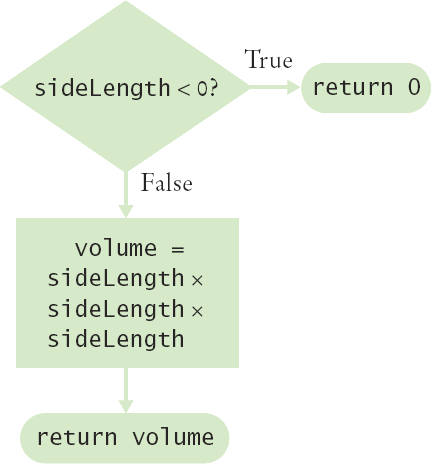
\includegraphics[height=0.5\paperheight,center]{pucrs-ep-fprog-unidade_05-metodos-laminas-fluxograma_return.png}
\end{figure}
	\end{column}
\end{columns}
\end{frame}

%-------------------------------------------------------
\begin{frame}[fragile]\frametitle{Erro Comum}
Erro comum = esquecer o comando \texttt{return}
\begin{itemize}
	\item Verifique se todas as condições estão sendo tratadas
	\item No exemplo abaixo, \texttt{x} poderia ser igual a 0 e não foi previsto um \texttt{return} para esta situação
	\item O compilador vai reclamar se algum \texttt{return} for esquecido
\begin{javacode}
public static int sign(double x) {
  if (x < 0) { return -1; }
  if (x > 0) { return 1; }
  // Erro: falta um valor a ser retornado se x for igual a 0
}
\end{javacode}
\end{itemize}
\end{frame}

%-------------------------------------------------------
\begin{frame}[fragile]\frametitle{Implementando um Método: Passos}
\begin{enumerate}
	\item Descreva o que o método deveria fazer
	\item Determine as entradas para o método
	\item Determine os tipos dos parâmetros e do valor de retorno
	\item Escreva pseudocódigo para obter o resultado desejado
	\item Implemente o corpo do método
\begin{javacode}
public static double pyramidVolume(double height, double baseLength) {
  double baseArea = baseLength * baseLength;
  return height * baseArea / 3;
}
\end{javacode}
	\item Teste o seu método: projete casos de teste
\end{enumerate}
\end{frame}

%=======================================================
\section{Métodos sem Retorno de Valores}

%-------------------------------------------------------
\begin{frame}[fragile]\frametitle{Métodos sem Retorno de Valores}
\begin{itemize}
	\item Métodos não necessitam retornar um valor
	\item O tipo de retorno \texttt{void} significa que nada será retornado
	\item Nenhum comando \texttt{return} é necessário
	\item O médoto pode gerar saída!
{\tiny
\begin{javacode}
public static void boxString(String str) {
  int n = str.length();
  for (int i = 0; i < n + 2; i++)  { System.out.print("-"); }
  System.out.println();
  System.out.println("!" + str + "!");
  for (int i = 0; i < n + 2; i++)  { System.out.print("-"); }
  System.out.println();
}
\end{javacode}
\begin{javacode}
...
boxString("Hello");
...
\end{javacode}
\begin{javacode}
-------
!Hello!
-------
\end{javacode}
}
\end{itemize}
\end{frame}

%-------------------------------------------------------
\begin{frame}[fragile]\frametitle{Usando \texttt{return} sem nenhum valor}
\begin{itemize}
	\item Você pode usar o comando \texttt{return} sem nenhum valor
	\item Em métodos com tipo de retorno \texttt{void}, o comando \texttt{return} encerra imediatamente o método
{\scriptsize
\begin{javacode}
public static void boxString(String str) {
  int n = str.length();
  if (n == 0) {
    return; // Return immediately
  }
  for (int i = 0; i < n + 2; i++) { System.out.print("-"); }
  System.out.println();
  System.out.println("!" + str + "!");
  for (int i = 0; i < n + 2; i++) { System.out.print("-"); }
  System.out.println();
}
\end{javacode}
}
\end{itemize}
\end{frame}

%=======================================================
\section{Exercícios}

%-------------------------------------------------------
\begin{frame}\frametitle{Exercícios}
Implemente métodos para os seguintes casos:
\begin{itemize}
	\item calcular as áreas de: quadrado, retângulo, círculo, trapézio, triângulo
	\item verificar se, dados 3 comprimentos, eles poderiam corresponder aos lados de um triângulo ou não
	\item calcular o fatorial de um número
	\item verificar se um número é primo ou não
        \item determinar se uma cadeia de caracteres é um palíndromo ou não (exemplos: "OVO" é palíndromo, "CASA" não é)
\end{itemize}
\end{frame}

\begin{comment}
%-------------------------------------------------------
\begin{frame}\frametitle{Exercícios (2)}
\begin{itemize}
	\item Implemente um método \texttt{multInt(int a, int b)} para calcular \texttt{a} multiplicado por \texttt{b} usando apenas somas sucessivas.
	\item Implemente um método \texttt{powInt(int a, int b)} para calcular \texttt{a} elevado na potência \texttt{b} usando apenas multiplicações sucessivas. Use o método \texttt{multInt}.
	\item Implemente um método \texttt{main} para testar o método \texttt{powInt} (e indiretamente também testar o método \texttt{multInt}).
\end{itemize}
\end{frame}
\end{comment}

%=======================================================
\section{Solução de Problemas: Reutilização de Métodos}

%-------------------------------------------------------
\begin{frame}[fragile]\frametitle{Solução de Problemas: Reutilização de Métodos}
\begin{itemize}
	\item Procure código ``repetido''
	\begin{itemize}
		\item Pode envolver valores diferentes, porém com a mesma lógica
\begin{javacode}
Scanner in = new Scanner(System.in);
int horas;
do {
   System.out.print("Digite um valor de 0 a 23: ");
   horas = in.nextInt();
}  while (horas < 0 || horas > 23);

int minutos;
do {
   System.out.print("Digite um valor de 0 a 59: ");
   minutos = in.nextInt();
}  while (minutos < 0 || minutos > 59);
\end{javacode}
	\end{itemize}
\end{itemize}
\end{frame}

%-------------------------------------------------------
\begin{frame}[fragile]\frametitle{Escreva um método parametrizado}
{\tiny
\begin{javacode}
/**
  Solicita que o usuario digite um valor, aceitando apenas
  valores em um intervalo predefinido.

  @param inf o limite inferior do intervalo
  @param sup o limite superior do intervalo
  @return o valor digitado pelo usuario
*/
public static int leiaValoresNoIntervalo(Scanner in, int inf, int sup) {
  int entrada;
  do {
     System.out.print("Digite um valor de " + inf + " a " + sup + ": ");
     entrada = in.nextInt();
  }  while (entrada < inf || entrada > sup);
  return entrada;
}

/* ... */

Scanner in = new Scanner(System.in);
int horas = leiaValoresNoIntervalo(in,0,23);
int minutos = leiaValoresNoIntervalo(in,0,59);
\end{javacode}
}
\end{frame}

%=======================================================
\section{Solução de Problemas: Refinamento Passo-a-passo}

%-------------------------------------------------------
\begin{frame}\frametitle{Solução de Problemas: Refinamento Passo-a-passo}
\begin{itemize}
	\item Refinamento de passos
	\begin{itemize}
		\item Para resolver uma tarefa difícil, decomponha ela em tarefas mais simples
		\item Então continue decompondo as tarefas simples em tarefas cada vez mais simples, até que você chegue a tarefas que você saiba como resolver
	\end{itemize}
\end{itemize}
\end{frame}

%-------------------------------------------------------
\begin{frame}\frametitle{Exemplo: Quer Tomar Café?}
\begin{itemize}
	\item Se você tiver que fazer um café, há duas opçôes:
	\begin{itemize}
		\item Faça um café instantâneo
		\item Passe um café
	\end{itemize}
\begin{figure}[h]
	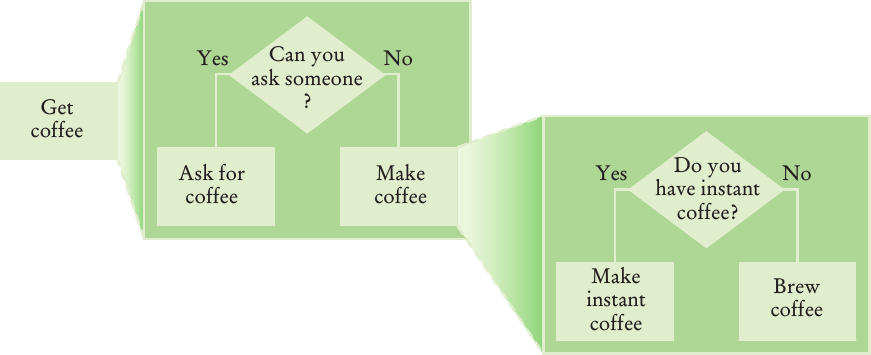
\includegraphics[height=0.50\paperheight,center]{pucrs-ep-fprog-unidade_05-metodos-laminas-get_coffe_1.png}
\end{figure}
\end{itemize}
\end{frame}

%-------------------------------------------------------
\begin{frame}\frametitle{Café Instantâneo}
\begin{columns}[T]
	\begin{column}{0.3\linewidth}
		\begin{itemize}
		\item Há duas formas de ferver a água:
		\begin{itemize}
			\item Use o microonddas
			\item Use uma chaleira no fogão
		\end{itemize}
		\end{itemize}
	\end{column}
	\begin{column}{0.7\linewidth}\begin{figure}[h]
	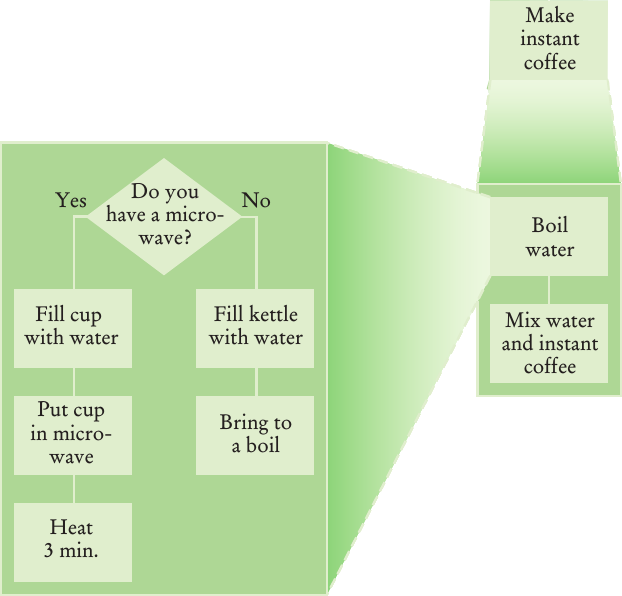
\includegraphics[height=0.65\paperheight,center]{pucrs-ep-fprog-unidade_05-metodos-laminas-get_coffe_2.png}
\end{figure}
	\end{column}
\end{columns}
\end{frame}

%-------------------------------------------------------
\begin{frame}\frametitle{Café Passado}
\begin{columns}[T]
	\begin{column}{0.3\linewidth}
		\begin{itemize}
		\item Considerando o uso de uma cafeteira:
		\begin{itemize}
			\item Adicione água
			\item Adicione o filtro
			\item Moa o café
			\begin{itemize}
				\item Adicione os grãos no moedor
				\item Moa por 60 segundos
			\end{itemize}
			\item Encha o filtro com o café moído
			\item Ligue a máquina de café
		\end{itemize}
		\end{itemize}
	\end{column}
	\begin{column}{0.7\linewidth}\begin{figure}[h]
	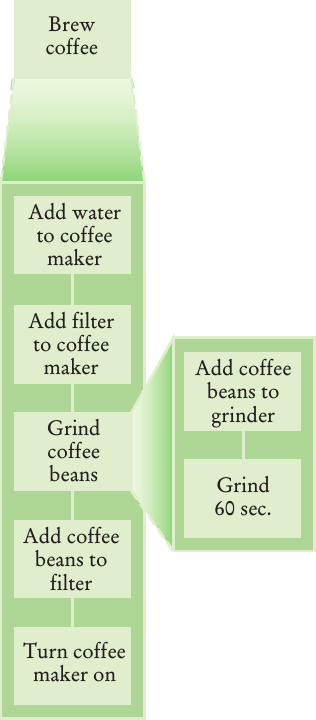
\includegraphics[height=0.65\paperheight,center]{pucrs-ep-fprog-unidade_05-metodos-laminas-get_coffe_3.png}
\end{figure}
	\end{column}
\end{columns}
\end{frame}

%-------------------------------------------------------
\begin{frame}\frametitle{Exemplo de Refinamento de Passos}
\begin{itemize}
	\item Quando se preenche um cheque, costuma-se preencher o valor total tanto no formato numérico (R\$274,15) quanto no formato textual (duzentos e setenta e quatro reais e quinze centavos). Escreva um programa para transformar um número em um texto.
	\item Mesmo que pareça difícil, pode-se iniciar fazendo algumas \textbf{simplificações} para a seguir \textbf{decompor} o problema
	\begin{itemize}
		\item Inicialmente separe a parte inteira (valor em reais sem centavos) e considere apenas valores de 0 até 999
		\item Analise a questão dígito por dígito: isole os dígitos para centenas, dezenas e unidades
		\item Você vai precisar de um método para resolver o problema (por exemplo, \texttt{numeroPorExtenso})
		\item Este método poderá usar métodos para cada tipo de dígito: \texttt{nomeCentena}, \texttt{nomeDezena} e \texttt{nomeUnidade}
		\item \textbf{Identifique e resolva as situações gerais, depois trate os casos específicos!}
	\end{itemize}
\end{itemize}
\end{frame}

%-------------------------------------------------------
\begin{frame}\frametitle{Tratando Centenas}
\begin{itemize}
	\item Método \texttt{nomeCentena}:
	\begin{itemize}
		\item Identifique todas as palavras envolvidas e também situações em que elas serão utilizadas
		\item Se não houver centena, não há nada a fazer
		\item Se a centena for igual a 1, há duas possibilidades
		\begin{itemize}
			\item Sem resto, a palavra é ``cem''
			\item Havendo resto, o texto deverá ser ``cento e ''
		\end{itemize}
		\item Para as outras centenas, os textos são bem comportados: ``duzentos'', ``trezentos'', ``quatrocentos'', etc.
		\begin{itemize}
			\item Havendo resto, após o texto deverá ser acrescentado `` e ''
		\end{itemize}
	\end{itemize}
\end{itemize}
\end{frame}

%-------------------------------------------------------
\begin{frame}\frametitle{Tratando Dezenas}
\begin{itemize}
	\item Método \texttt{nomeDezena}:
	\begin{itemize}
		\item Identifique todas as palavras envolvidas e também situações em que elas serão utilizadas
		\item Se não houver dezena, não há nada a fazer
		\item Se a dezena for igual a 1, dezena e resto devem ser tratados de forma unificada, então é melhor fazer isto no método das unidades
		\item Para as outras dezenas, os textos são bem comportados: ``vinte'', ``trinta'', ``quarenta'', etc.
		\begin{itemize}
			\item Havendo resto, após o texto deverá ser acrescentado `` e ''
		\end{itemize}
	\end{itemize}
\end{itemize}
\end{frame}

%-------------------------------------------------------
\begin{frame}\frametitle{Tratando Unidades}
\begin{itemize}
	\item Método \texttt{nomeUnidade}:
	\begin{itemize}
		\item Identifique todas as palavras envolvidas e também situações em que elas serão utilizadas
		\item Se não houver unidade, não há nada a fazer
		\item Se houver unidade, os textos são: ``um'', ``dois'', ``tres'', ``quatro'', etc.
		\item Este método também tratará as dezenas como se fossem unidades, portanto, também haverá textos para: ``dez'', ``onze'', ``doze'', ``treze'', ``catorze'', etc.
	\end{itemize}
\end{itemize}
\end{frame}

%-------------------------------------------------------
\begin{frame}\frametitle{Tratando o Zero}
\begin{itemize}
	\item 0 (``zero'') é um caso especial e deve ser tratado à parte
\end{itemize}
\end{frame}

%-------------------------------------------------------
\begin{frame}[fragile]\frametitle{Escreva Pseudocódigo}
{\tiny
\begin{verbatim}
numero = n (numero a ser convertido)
texto  = "" (texto correspondente ao numero)
se numero for 0 entao texto = "zero"
senao
inicio
  // calcula numero de centenas, dezenas e unidades
  centenas = numero / 100
  restoCentenas = numero % 100
  dezenas = restoCentenas / 10
  unidades = restoCentenas % 10

  // trata dezenas como unidades
  se dezenas for igual a 1
  entao inicio
          dezenas = 0
          unidades = unidades + 10
        fim

  // gera resultado
  texto = nomeCentena(centenas,restoCentenas) + nomeDezena(dezenas,unidades) + nomeUnidade(unidades)
fim
\end{verbatim}
}
\end{frame}

%-------------------------------------------------------
\begin{frame}\frametitle{Planeje os Métodos}
\begin{itemize}
	\item \texttt{main} chama \texttt{numeroPorExtenso}
	\item \texttt{numeroPorExtenso} faz todo o trabalho retornando um \texttt{String}
	\item \texttt{numeroPorExtenso} usa os métodos \texttt{nomeCentena}, \texttt{nomeDezena} e \texttt{nomeUnidade}
	\item \texttt{nomeCentena} recebe o número de centenas e o resto, retornando um \texttt{String}
	\item \texttt{nomeDezena} recebe o número de dezenas e o resto, retornando um \texttt{String}
	\item \texttt{nomeUnidade} recebe o número de unidades, retornando um \texttt{String}
\end{itemize}
\end{frame}

%-------------------------------------------------------
\begin{frame}[fragile]\frametitle{Dicas de Programação}
\begin{itemize}
	\item Mantenha os métodos pequenos: se ficarem maiores do que uma página, quebre eles em submétodos
	\item Execute seus métodos manualmente, mostrando a evolução da alteração das variáveis
	\begin{itemize}
		\item Use linhas para cada passo e reserve colunas para as variáveis importantes 
	\end{itemize}
\begin{figure}[h]
	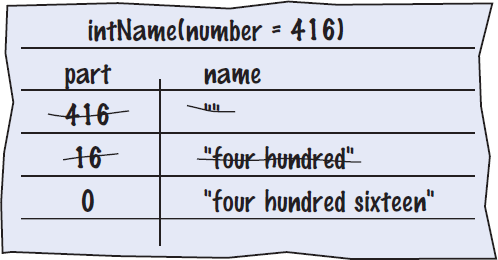
\includegraphics[height=0.15\paperheight,center]{pucrs-ep-fprog-unidade_05-metodos-laminas-teste_de_mesa.png}
\end{figure}
	\item Use métodos incompletos, com conteúdo provisório, que retornam valores ``fictícios'' durante o desenvolvimento
\begin{javacode}
public static String nomeUnidade(int unidades) {
   return "unidade";
}
\end{javacode}
\end{itemize}
\end{frame}

%=======================================================
\section{Escopo de Variáveis}

%-------------------------------------------------------
\begin{frame}\frametitle{Escopo de Variáveis}
\begin{itemize}
	\item Variáveis podem ser declaradas
	\begin{itemize}
		\item Dentro de um método
		\begin{itemize}
			\item Chamadas de ``variáveis locais'' (ou de escopo local)
			\item Somente podem ser acessadas dentro do método
			\item Variáveis paramétricas são deste tipo
		\end{itemize}
		\item Dentro de um bloco de código \textbf{\{\}}
		\begin{itemize}
			\item Chamadas de ``variáveis de bloco'' (ou de escopo de bloco)
			\item Não podem ser acessadas depois do fim do bloco
		\end{itemize}
		\item Fora de um método
		\begin{itemize}
			\item Chamadas de ``variáveis globais'' (ou de escopo global)
			\item Podem ser usadas (e alteradas) por código em qualquer método
		\end{itemize}
	\end{itemize}
	\item O escopo de uma variável corresponde à parte do programa onde ela é visível
	\item Como escolher? Qual a melhor forma?
\end{itemize}
\end{frame}

%-------------------------------------------------------
\begin{frame}[fragile]\frametitle{Exemplo de Escopo}
\begin{itemize}
	\item \texttt{sum} é uma variável local em \texttt{main}
	\item \texttt{square} é visível apenas dentro do bloco do laço \texttt{for}
	\item \texttt{i} é visível apenas dentro do laço \texttt{for}
\begin{javacode}
public static void main(String[] args) { // ESCOPOS:
  int sum = 0;                           // sum
  for (int i = 1; i <= 10; i++)  {       // sum, i
    int square = i * i;                  // sum, i, square
    sum = sum + square;                  // sum, i, square
  }                                      // sum
  System.out.println(sum);               // sum
}                                        //
\end{javacode}
\end{itemize}
\end{frame}

%-------------------------------------------------------
\begin{frame}[fragile]\frametitle{Variáveis Locais de Métodos}
\begin{itemize}
	\item Variáveis declaradas dentro de um método \textbf{não} são visíveis a outros métodos
	\begin{itemize}
		\item \texttt{sideLength} é local do método \texttt{main}
		\item Usá-la fora do método causará um erro de compilação
	\end{itemize}
\begin{javacode}
public static void main(String[] args) {
  double sideLength = 10;
  int result = cubeVolume();
  System.out.println(result);
}

public static double cubeVolume() {
  return sideLength * sideLength * sideLength; // ERROR
}
\end{javacode}
\end{itemize}
\end{frame}

%-------------------------------------------------------
\begin{frame}[fragile]\frametitle{Reutilização de Nomes de Variáveis Locais}
\begin{itemize}
	\item Variáveis declaradas dentro de um método \textbf{não} são visíveis a outros métodos
	\begin{itemize}
		\item \texttt{result} é local de \texttt{square} e \texttt{result} também é local em \texttt{main}
		\item São duas variáveis diferentes que não se sobrepõem
	\end{itemize}
\begin{javacode}
public static int square(int n) {
  int result = n * n;
  return result;
}

public static void main(String[] args) {
  int result = square(3) + square(4);
  System.out.println(result);
}
\end{javacode}
\end{itemize}
\end{frame}

%-------------------------------------------------------
\begin{frame}[fragile]\frametitle{Reutilização de Nomes de Variáveis de Blocos}
\begin{itemize}
	\item Variáveis declaradas dentro de um bloco \textbf{não} são visíveis a outros blocos
	\begin{itemize}
		\item \texttt{i} está dentro do primeiro bloco e \texttt{i} também está dentro do segundo bloco
		\item São duas variáveis diferentes que não se sobrepõem
	\end{itemize}
\begin{javacode}
public static void main(String[] args) {
  int sum = 0;
  for (int i = 1; i <= 10; i++) {
    sum = sum + i;
  }
  for (int i = 1; i <= 10; i++) {
    sum = sum + i * i;
  }
  System.out.println(sum);
}
\end{javacode}
\end{itemize}
\end{frame}

%-------------------------------------------------------
\begin{frame}[fragile]\frametitle{Escopos Sobrepostos}
\begin{itemize}
	\item Variáveis (incluindo variáveis paramétricas) devem ter nomes únicos dentro de seu escopo
	\begin{itemize}
		\item \texttt{n} tem escopo local e \texttt{n} está declarado em um bloco dentro deste escopo
		\item O compilador vai reclamar quando a variável \texttt{n} for declarada no escopo do bloco
	\end{itemize}
\begin{javacode}
public static int sumOfSquares(int n) { // ESCOPOS:
  int sum = 0;                          // n
  for (int i = 1; i <= n; i++) {        // n
    int n = i * i; /* ERRO */           // n, n
    sum = sum + n;                      // n, n
  }                                     // n
  return sum;                           // n
}
\end{javacode}
\end{itemize}
\end{frame}

%-------------------------------------------------------
\begin{frame}[fragile]\frametitle{Sobreposição Global e Local}
\begin{itemize}
	\item Variáveis globais e locais (de métodos) podem se sobrepor
	\begin{itemize}
		\item A variável local \texttt{same} será usada no seu contexto local
		\item Não há acesso à variável global \texttt{same} quando \texttt{same} local estiver em seu escopo
	\end{itemize}
{\scriptsize
\begin{javacode}
public class Scoper {                       // ESCOPOS:
  public static int same; /* global */      // same
  public static void main(String[] args) {  // same
    int same = 0; /* local */               // same, same
    for (int i = 1; i <= 10; i++) {         // same, same
      int square = i * i;                   // same, same
      same = same + square;                 // same, same
    }                                       // same, same
    System.out.println(same);               // same
  }
}
\end{javacode}
}
	\item Variáveis com o mesmo nome em diferentes escopos não geram erro de compilação, mas não é uma boa ideia fazer isto
\end{itemize}
\end{frame}

%-------------------------------------------------------
\begin{frame}[fragile]\frametitle{Exercício 1}
Considere o programa em Java a seguir e mostre o que será impresso, respeitando a ordem de execução.
\begin{columns}[T]
	\begin{column}{0.5\linewidth}
{\tiny
\begin{javacode}
public class Teste1 {
    public static int a = 9;
    public static int b = 21;
    
    public static int metodo1(int b) {
        b++;
        System.out.println("[1] "+a);
        System.out.println("[2] "+b);
        int a = 5;
        a *= 3;
        System.out.println("[3] "+a);
        return a;
    }
    
    public static int metodo2(int a) {
        System.out.println("[4] "+a);
        System.out.println("[5] "+b);
        int b = (a%2==0)?1:0;
        System.out.println("[6] "+b);
        return b;
    }
\end{javacode}
}
	\end{column}
	\begin{column}{0.5\linewidth}
{\tiny
\begin{javacode}
    public static void main(String[] args) {
        a++;
        b--;
        System.out.println("[7] "+a);
        System.out.println("[8] "+b);
        int a = metodo1(b);
        int b = metodo2(a);
        System.out.println("[9] "+a);
        System.out.println("[10] "+b);
        System.out.println("[11] "+Teste1.a);
        System.out.println("[12] "+Teste1.b);
    }    
}
\end{javacode}
}
	\end{column}
\end{columns}
\end{frame}

%-------------------------------------------------------
\begin{frame}[fragile]\frametitle{Exercício 2}
For each of the variables in the following program, indicate the scope. Then determine what the program prints, without actually running the program. (HORSTMANN, 2013, p. 237)
\begin{columns}[T]
	\begin{column}{0.5\linewidth}
{\scriptsize
\begin{javacode}
public class Sample {

    public static void main(String[] args) {
        int i = 10;
        int b = g(i);
        System.out.println(b + i);
    }

    public static int f(int i) {
        int n = 0;
        while (n * n <= i) { n++; }
        return n - 1;
    }
\end{javacode}
}
	\end{column}
	\begin{column}{0.5\linewidth}
{\scriptsize
\begin{javacode}
    public static int g(int a) {
        int b = 0;
        for (int n = 0; n < a; n++) {
            int i = f(n);
            b = b + i;
        }
        return b;
    }
}
\end{javacode}
}
	\end{column}
\end{columns}
\end{frame}

%=======================================================
\section{Métodos Recursivos}

%-------------------------------------------------------
\begin{frame}\frametitle{Métodos Recursivos}
\begin{itemize}
	\item Um método recursivo é um método que chama a si mesmo
	\item Uma computação recursiva resolve um problema dividindo o problema em computações mais simples e aplicando essa mesma estratégia sobre estas computações mais simples
	\item Para uma recursão terminar, deve haver pelo menos um caso especial para essas entradas mais simples
	\item Métodos recursivos são comuns na matemática - o fatorial é um exemplo:
    \begin{itemize}
        \item Fatorial de $0$ e de $1$ é por definição $1$: ~ ~ ~ ~ ~ ~ ~ ~ ~ ~ ~$0! = 1$ e $1! = 1$
        \item Fatorial de $n$ é igual a $n$ vezes o fatorial de $n-1$: ~ ~ $n! = n \times (n-1)!$
    \end{itemize}
\end{itemize}
\end{frame}

%-------------------------------------------------------
\begin{frame}[fragile]\frametitle{Exemplo: Triângulo Recursivo}
\begin{columns}[T]
	\begin{column}{0.5\linewidth}
\begin{itemize}
    \scriptsize
	\item O médoto chama a si mesmo (e não mostra nada) até que \texttt{tam} seja menor do que $1$
	\item Neste caso, ele usa o comando \texttt{return} e todas as iterações anteriores imprimem os seus resultados: 1, 2, 3, 4
\begin{javacode}
public static void triangulo(int tam) {
  if (tam < 1)
     return;
  triangulo(tam - 1);
  for (int i = 0; i < tam; i++)
    System.out.print("*");
  System.out.println();
}
\end{javacode}
\end{itemize}
	\end{column}
	\begin{column}{0.5\linewidth}
{\scriptsize
\begin{itemize}
    \scriptsize
    \item Aqui está o que acontece quando se manda imprimir um triângulo com tamanho igual a 4:
    \begin{itemize}
    \scriptsize
	\item A chamada \texttt{triangulo(4)} chama \texttt{triangulo(3)}
	\item A chamada \texttt{triangulo(3)} chama \texttt{triangulo(2)}
	\item A chamada \texttt{triangulo(2)} chama \texttt{triangulo(1)}
	\item A chamada \texttt{triangulo(1)} chama \texttt{triangulo(0)}
	\item A chamada \texttt{triangulo(0)} retorna, sem fazer nada
	\item A chamada \texttt{triangulo(1)} imprime \texttt{*}
	\item A chamada \texttt{triangulo(2)} imprime \texttt{**}
	\item A chamada \texttt{triangulo(3)} imprime \texttt{***}
	\item A chamada \texttt{triangulo(4)} imprime \texttt{****}
    \end{itemize}
\end{itemize}
}
	\end{column}
\end{columns}
\end{frame}

%-------------------------------------------------------
\begin{frame}[fragile]\frametitle{Recursão}
\begin{itemize}
    \item Quando chamamos um método, o código que fez a chamada fica esperando até a chamada do método seja concluída
    \item Na execução de um método recursivo, acontece a mesma coisa
    \begin{itemize}
        \item Temos instâncias do método esperando que outras instâncias do mesmo método terminem
        \item A chamada que foi executada antes aguarda que a chamada que ela fez termine - e isso acontece de forma encadeada
    \end{itemize}
    \item Em algum momento, o método recursivo precisa parar de se invocar, pois senão teríamos uma espécie de laço infinito
    \item Para evitar problemas de inconsistência, métodos recursivos devem evitar acessar variáveis globais
    \item De forma geral, se temos um problema resolvido com laços aninhados, a versão recursiva consegue eleminar um nível de laços
\end{itemize}
\end{frame}

%-------------------------------------------------------
\begin{frame}\frametitle{Exercício 1}
Implemente funções recursivas para:
\begin{enumerate}
	\item Fatorial de $n$
    \begin{itemize}
        \item $fatorial(0) = 1$
        \item $fatorial(1) = 1$
        \item $fatorial(n) = n \times fatorial(n-1)$
    \end{itemize}
	\item Número de Fibonacci de ordem $n$
	\begin{itemize}
        \item $fibonacci(0) = 0$
        \item $fibonacci(1) = 1$
        \item $fibonacci(n) = fibonacci(n-1) + fibonacci(n-2)$
    \end{itemize}
	\item Imprimir os números inteiros de 1 até $n$, inclusive.
	\item Imprimir os números inteiros de $n$ até 1, inclusive.
	%\item Imprimir os números inteiros de $a$ até $b$, com incremento $r$, considerando $a \leqslant b$ e $r > 0$.
\end{enumerate}
\end{frame}

%-------------------------------------------------------
\begin{frame}[fragile]\frametitle{Exercício 2}
Considere o programa em Java a seguir e mostre o que será impresso, respeitando a ordem de execução.
\begin{columns}[T]
	\begin{column}{0.5\linewidth}
{\tiny
\begin{javacode}
public class Teste2 {
    public static int a = 2;
    public static int b = 10;
    
    public static void metodo1(int b) {
        System.out.println("[1] "+a);
        int a = b;
        System.out.println("[2] "+a);
        if (b==1)
            return;
        else
            metodo1(b-1);
    }
\end{javacode}
}
	\end{column}
	\begin{column}{0.5\linewidth}
{\tiny
\begin{javacode}
    public static void metodo2() {
        System.out.println("[3] "+a);
        System.out.println("[4] "+b);
        metodo1(a);
        ++b;
        int b = 2;
        System.out.println("[5] "+a);
        System.out.println("[6] "+b);        
    }

    public static void main(String[] args) {
        System.out.println("[7] "+a);
        a++;
        int a = 15;
        System.out.println("[8] "+a);
        a++;
        metodo2();
        System.out.println("[9] "+a);        
    }    
}
\end{javacode}
}
	\end{column}
\end{columns}
\end{frame}

%=======================================================
\section{Sumário}

%-------------------------------------------------------
\begin{frame}\frametitle{Sumário: Métodos}
\begin{itemize}
	\item Um método é um nome para uma sequência de instruções
	\item Argumentos são fornecidos quando um método é chamado. O valor de retorno é o resultado que o método computa
	\item Quando se declara um método, deve-se prover um nome para o método, uma variável para cada argumento, e um tipo para o resultado
	\item Comentários de métodos explicam o propósito do método, o significado dos parâmetros e o valor de retorno, bem como qualquer requisito especial
    \begin{itemize}
		\item Sempre escreva uma descrição de cada variável paramétrica e do valor de retorno
    \end{itemize}
	\item Variáveis paramétricas armazenam os argumentos fornecidos na chamada do método
\end{itemize}
\end{frame}

%-------------------------------------------------------
\begin{frame}\frametitle{Sumário: Retornos de Métodos}
\begin{itemize}
	\item O comando \texttt{return} termina a execução de um método e especifica o resultado calculado pelo método
	\begin{itemize}
		\item Coloque computações que podem ser necessárias mais de uma vez dentro de métodos
		\item Use o tipo \texttt{void} para indicar que o método não retorna nenhum valor
	\end{itemize}
	\item Use o processo de refinamento passo-a-passo para decompor tarefas complexas em tarefas mais simples
	\begin{itemize}
		\item Um método pode necessitar de outros métodos mais simples para executar o seu trabalho
	\end{itemize}
\end{itemize}
\end{frame}

%-------------------------------------------------------
\begin{frame}\frametitle{Sumário: Escopo}
\begin{itemize}
	\item O escopo de uma variável é a parte do programa em que ela é visível
	\begin{itemize}
		\item Duas variáveis locais ou paramétricas podem ter o mesmo nome desde que seus escopos não se sobreponham
		\item Pode-se usar o mesmo nome de variável dentro de diferentes métodos desde que seus escopos não se sobreponham
		\item Variáveis locais declaradas dentro de um método não são visíveis ao código dentro de outros métodos
	\end{itemize}
\end{itemize}
\end{frame}

%-------------------------------------------------------
\begin{frame}\frametitle{Sumário: Recursão}
\begin{itemize}
	\item Uma computação recursiva soluciona um problema usando a solução do mesmo problema com entradas mais simples
	\begin{itemize}
		\item Para uma recursão encerrar, deve haver um caso especial para as entradas mais simples
		\item A chave para encontrar uma solução recursiva é reduzir a entrada para uma entrada mais simples para o mesmo problema
		\item Quando se projeta uma solução recursiva, não se preocupe com múltiplas chamadas aninhadas. Simplesmente mantenha o foco em reduzir o problema para uma forma mais simples
	\end{itemize}
\end{itemize}
\end{frame}

%=======================================================
\section{Exercícios}

%-------------------------------------------------------
\begin{frame}[fragile]\frametitle{Exercício 1}
{\scriptsize
Escreva os seguintes metodos em Java e teste-os em um método main():
\begin{itemize}
\item \texttt{double smallest(double x, double y, double z)}, retornando o menor valor entre todos os argumentos (por exemplo, \texttt{smallest(0,-1, 3.45)} retorna \texttt{-1.0000})
\item \texttt{double average(double x, double y, double z)}, retornando o valor medio de todos os argumentos (por exemplo, \texttt{average(1, 2, 6)} retorna \texttt{3.0000})
\item \texttt{boolean allTheSame(double x, double y, double z)}, retornando \texttt{true} se todos forem iguais, ou \texttt{false} em caso contrario (por exemplo, \texttt{allTheSame(1,1,1)} retorna \texttt{true} e \texttt{allTheSame(2,2,2.1)} retorna \texttt{false})
\item \texttt{boolean allDifferent(double x, double y, double z)}, retornando \texttt{true} se todos forem diferentes, ou \texttt{false} em caso contrario (por exemplo, \texttt{allDifferent(1,2,3)} retorna \texttt{true} e \texttt{allDifferent(1,1,2)} retorna \texttt{false})
\item \texttt{boolean sorted(double x, double y, double z)}, retornando \texttt{true} se os argumentos estiverem ordenados (\texttt{x}$\leqslant$\texttt{y}$\leqslant$\texttt{z}), ou \texttt{false} em caso contrario (por exemplo, \texttt{sorted(1,3,5)} retorna \texttt{true} e \texttt{sorted(1,3,2)} retorna \texttt{false})
\item \texttt{int firstDigit(int n)}, retornando o primeiro digito do argumento (por exemplo, \texttt{firstDigit(1729)} retorna \texttt{1})
\item \texttt{int lastDigit(int n)}, retornando o ultimo digito do argumento (por exemplo, \texttt{lastDigit(1729)} retorna \texttt{9})
\item \texttt{int digits(int n)}, retornando o numero de digitos do argumento (por exemplo, \texttt{digits(1729)} retorna \texttt{4})
\end{itemize}
}
\end{frame}

%-------------------------------------------------------
\begin{frame}[fragile]\frametitle{Exercício 2}
Implemente em Java dois métodos, um não recursivo e outro recursivo, que recebam um valor inteiro n e retornem o valor real correspondente ao n-ésimo número harmônico.
O número. O n-ésimo número harmônico, H(n), com n maior ou igual a 1, pode ser calculado da seguinte forma:
\[ H(n) = 1 + \frac{1}{2} + \frac{1}{3} +\frac{1}{4} + ... + \frac{1}{n}\]
\end{frame}

%=======================================================
\section{Referências}

%-------------------------------------------------------
\begin{frame}\frametitle{Referências}
\noindent{HORSTMANN, C. \textbf{Java for Everyone – Late Objects}. 2. ed. Hoboken: Wiley, 2013. xxxiv, 589 p.}
\end{frame}

%=======================================================
\end{document}

